\chapter{Perspectives}

My research outlook over the coming decade is going to shift away from studying the Earth's deep interior and move towards the surface. In the next century run-off, which drives fluvial erosion, will likely change significantly due to the effects of global warming on the Earth system. To quote the IPCC's Fifth Assessment Report \cite{IPCC-policy-2014}:

\begin{displayquote}
In many regions, changing precipitation or melting snow and ice are altering hydrological systems, affecting water resources in terms of quantity and quality (medium confidence). Glaciers continue to shrink almost worldwide due to climate change (high confidence), affecting run-off and water resources downstream (medium confidence). Climate change is causing permafrost warming and thawing in high-latitude regions and in high-elevation regions (high confidence).
\end{displayquote}

The impact of such change on sediment storage and transport is uncertain. We can look to the past for evidence of how fluvial systems have responded, but at a time scale of hundreds of years it can become difficult to distinguish the importance of events such as individual storms. Furthermore, as I will expand upon below, there is a broad range of different numerical models developed to study landscape change on different time and spatial scales. One key process is being overlooked: groundwater. Beyond simple empirical laws for 1D infiltration, no numerical models to my knowledge include the impact of groundwater flow on the evolution of fluvial erosion and deposition. Yet rivers recharge by not only by surface run-off but from the ground \citep[e.g.][]{condon-etal-2020}, and river networks most likely grow as a network within the partially saturated ground \citep[e.g.][]{devauchelle-etal-2017}. The challenge is to translate this concept into a testable model that can be applied to fluvial systems.

\section{Short-Term Research Perspectives}

Landscape evolution modelling on geological time-scales ($>10^{4}$\,yr) has been dominated by one single equation: the stream power law \citep[see][]{howard-1983,howard-1994}. If I return to the simple D diagram of surface processes (Figure \ref{ch2:1dmodel}), the stream power law makes one very sweeping assumption: the rate of change in sediment thickness within the landscape is zero, which is to say all sediment created is transported out of the model domain. Furthermore, assuming surface flow is the primary driver of landscape erosion and that positive $x$ is in the downstream direction then erosion, $E$, as a function of the power of the flow to detach particles of rock per unit width can be written as,
\begin{equation}
E = -k_{b}\rho_{w}gq_{w}^{m}\left(\partial_{x}z\right)^{n},
\label{eq:streampower-inv}
\end{equation}
where $k_{b}$ is a dimensional constant that parametrises bedrock erodability (\citealp{howard-1983}; units (m$^{2}$\,yr$^{-1}$)$^{1-m}$\,yr\,kg$^{-1}$), $\rho_{w}$ is water density, $g$ is gravity, $q_{w}$ is water flux per unit width (units m$^{2}$\,yr$^{-1}$),  $m$ and $n$ are constants. The exponent $m \sim 0.5$, as it is a function of how the stream flow width is proportional to the water flux \citep[e.g.][]{lacey-1930,leopold-1953,whittaker-etal-2007}. The exponent $n>0$ acts upon the slope. In two dimensions the change in elevation is then given by,
\begin{equation}
\partial_{t}z = U + kq_{w}^{m}\left(\partial_{x}z\right)^{n},
\label{eq:streampower}
\end{equation}
where the constant $k$ lumps together the other constants (units m$^{-1}$\,(m$^{2}$\,yr$^{-1}$)$^{1-m}$), and if $n\neq1$ equation \ref{eq:streampower} becomes non-linear. But in any landscape, the assumption of instantaneous sediment transport does not hold. The above model does not work. This raises a question: {\bf what are the key processes within landscape evolution?}

Process based landscape evolution models (LEMs) have been created for various applications \citep[see for example][]{temme-etal-2017}. I will briefly describe two that have been used to study landscape change over different time-scales:
\begin{itemize}
\item[1] {\bf LAPSUS}
This is a process based model, where sediment is eroded or deposited down slope based on the transport capacity of the fluvial system \citep{schoorl-etal-2000}. It also includes processes such as soil formation and solid creep. It is a highly simplistic model with eight free parameters which can vary in space and time.
\item[2] {\bf CAESAR-Lisflood}
This is a process based model but of increased complexity compared to LAPSUS. It is based on a cellular automaton approach, but the laws acting on each cell are many and complex. Overland flow is modelled using the Lisflood model of \cite{bates-etal-2010}, and a simple infiltration is included using TOPMODEL \citep{beven-1979}. Subsequently sediment is transported down slope given the shear velocity of the flow is sufficiently high \citep{coulthard-etal-2013,vandeweil-etal-2007}. Other processes are included such as soil creation, lateral erosion, vegetation cover, etc., giving a total of 49 free parameters \citep{skinner-etal-2018}.
\item[3] {\bf DionisosFlow}
This software began as a a relatively simple model that solved for sediment transport solving a set of continuum equations \citep{granjeon-1999}. Since its conception it has grown it a set of modules that can include weathering, soil creation, infiltration, and carbonate formation, whilst still solving for a set of coupled equations \citep{peton-etal-2020}. The complexities of the possible output stratigraphy generated by this model has been used to argue that solutions for landscape evolution are non-unique \citep{burgess-2015}.
\end{itemize}
Given the number of processes typically modelled in LEMs it is difficult to assess which are significant and those to which there is no sensitivity. Recently sensitivity analysis has been carried for CAESAR-Lisflood out using a part of the full parameter space \citep{skinner-etal-2018}. The result of this sensitivity analysis is that the greatest sensitivity was to the sediment transport law, which is a function of the flow of water. This is arguably a first order variable within the model, and it suggests second order aspects such as the degree of vegetation, soil creation are of lower importance.

\begin{figure}
\begin{minipage}{\textwidth}
\begin{minipage}{.5\textwidth}
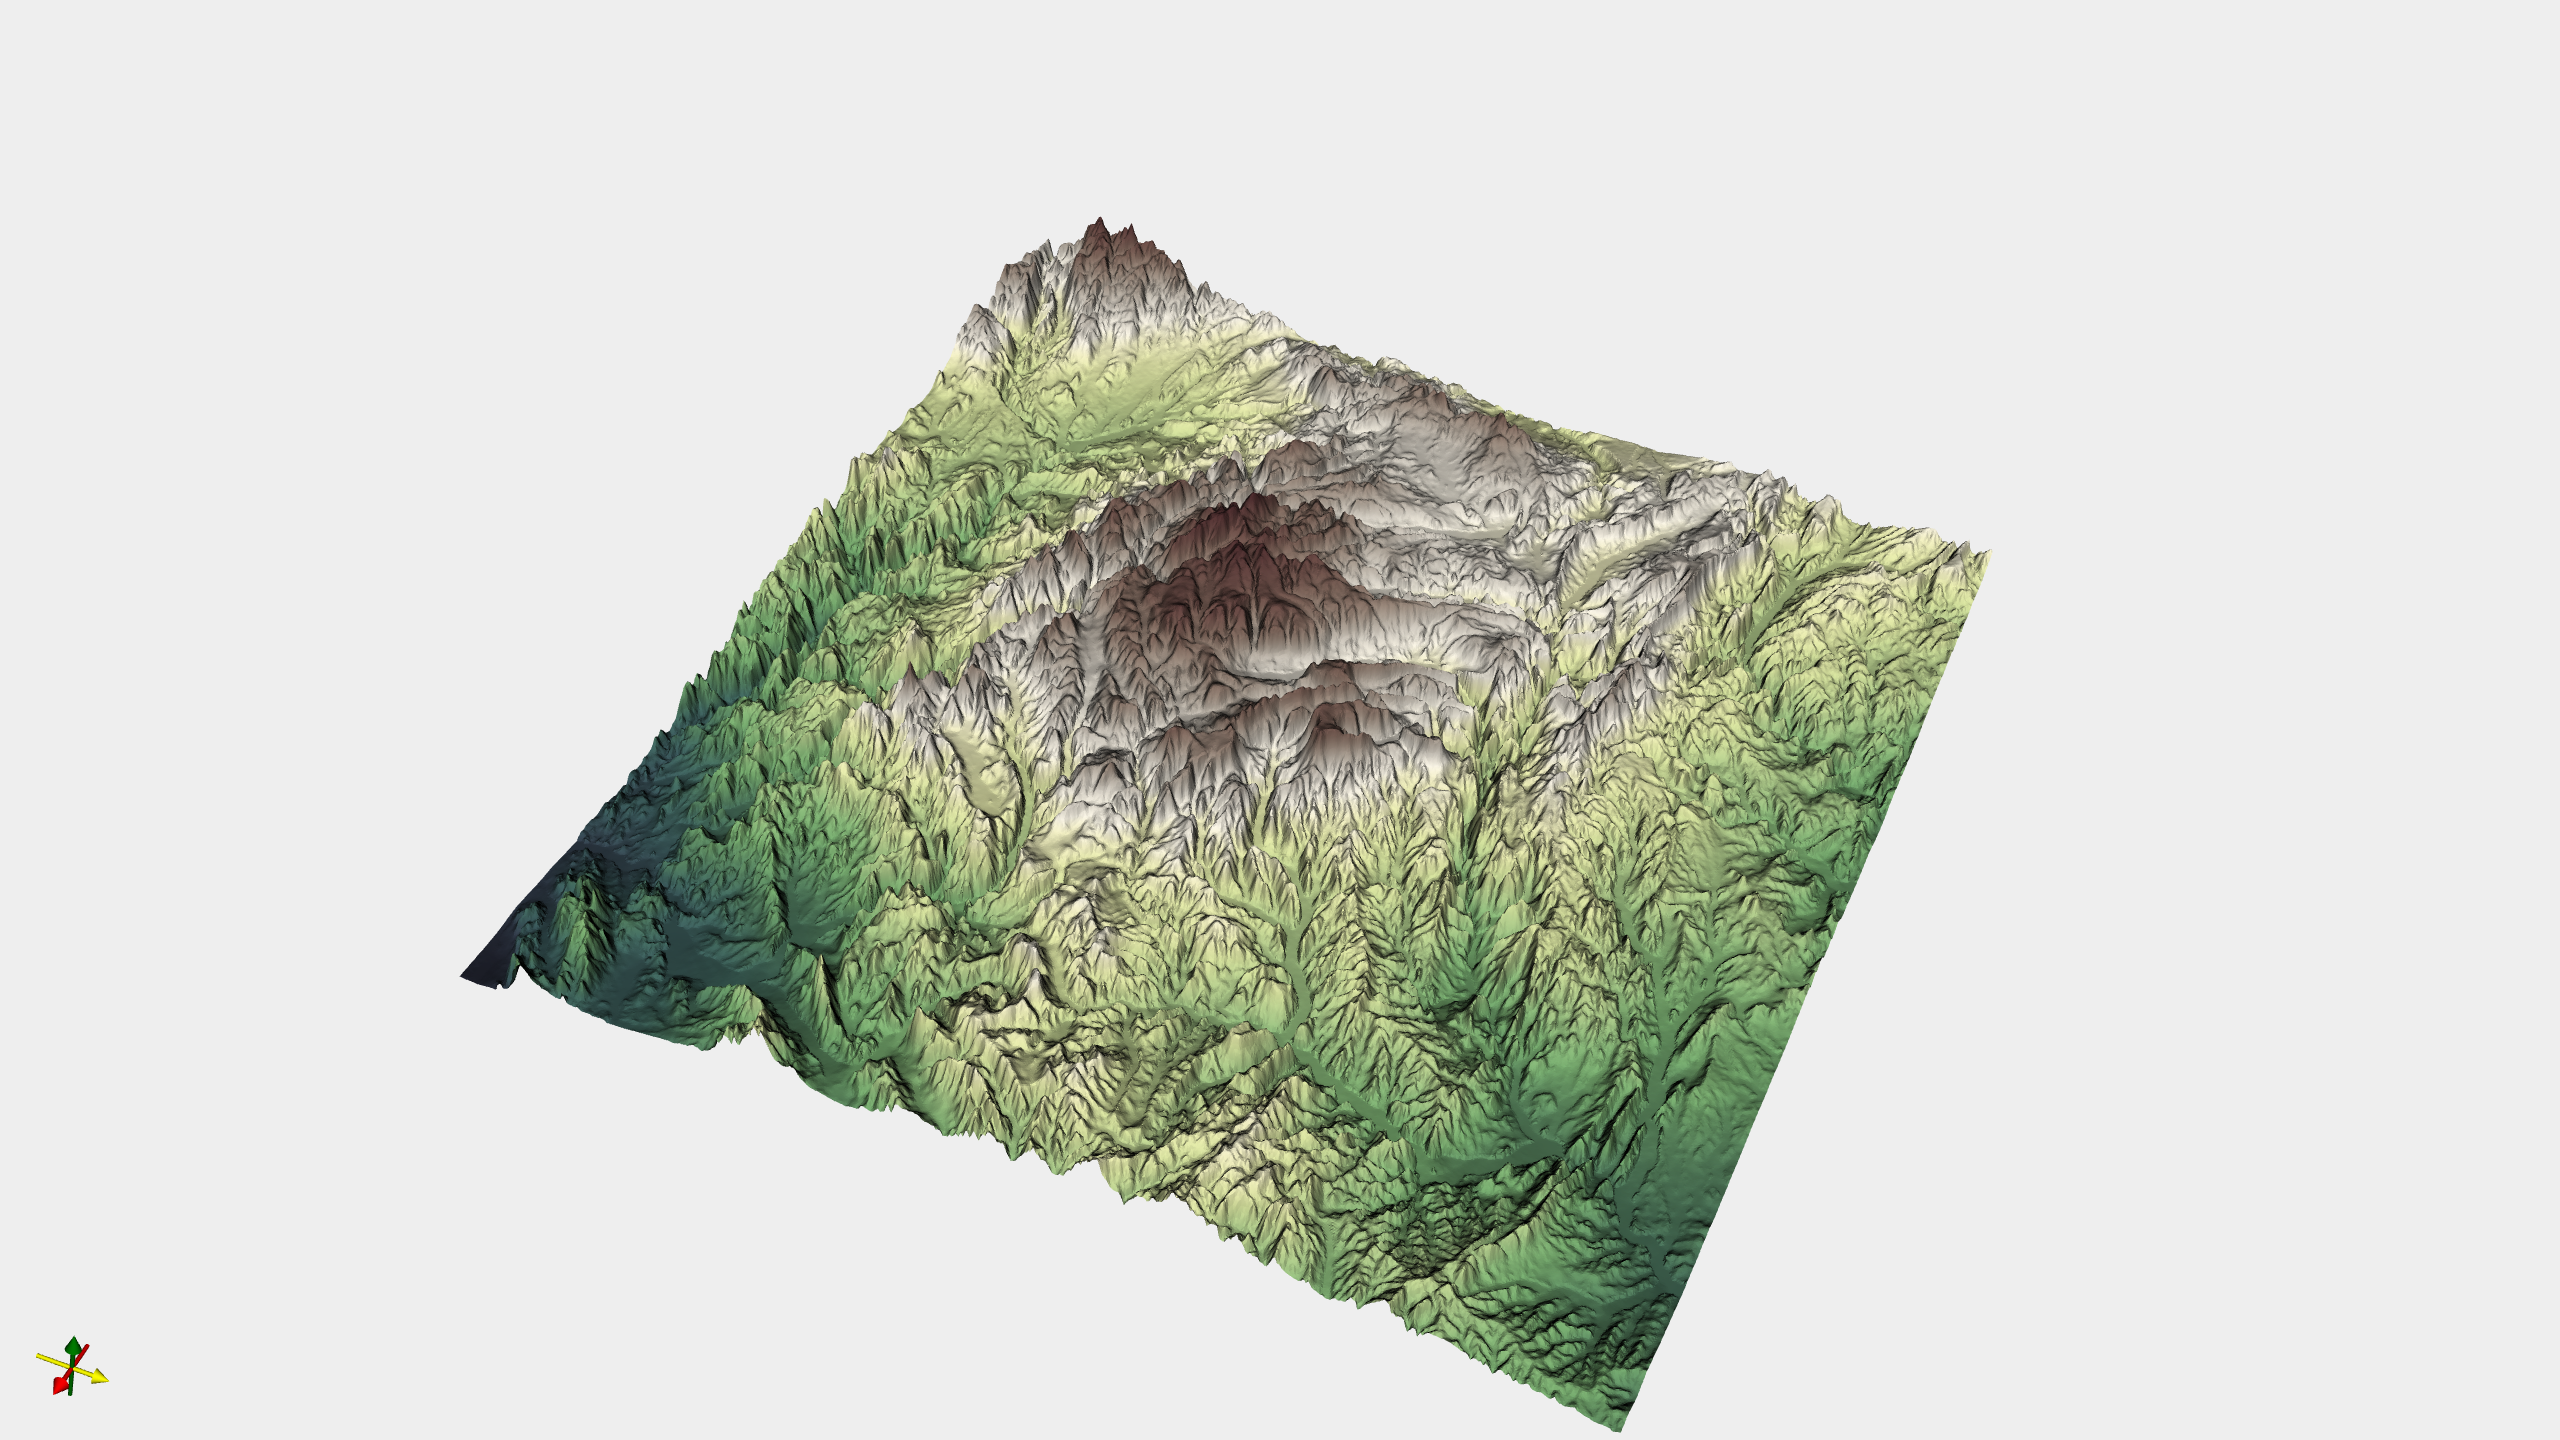
\includegraphics[width=.98\textwidth]{./figures/ch3-bergantes-elevation.png}
\end{minipage}
\begin{minipage}{.5\textwidth}
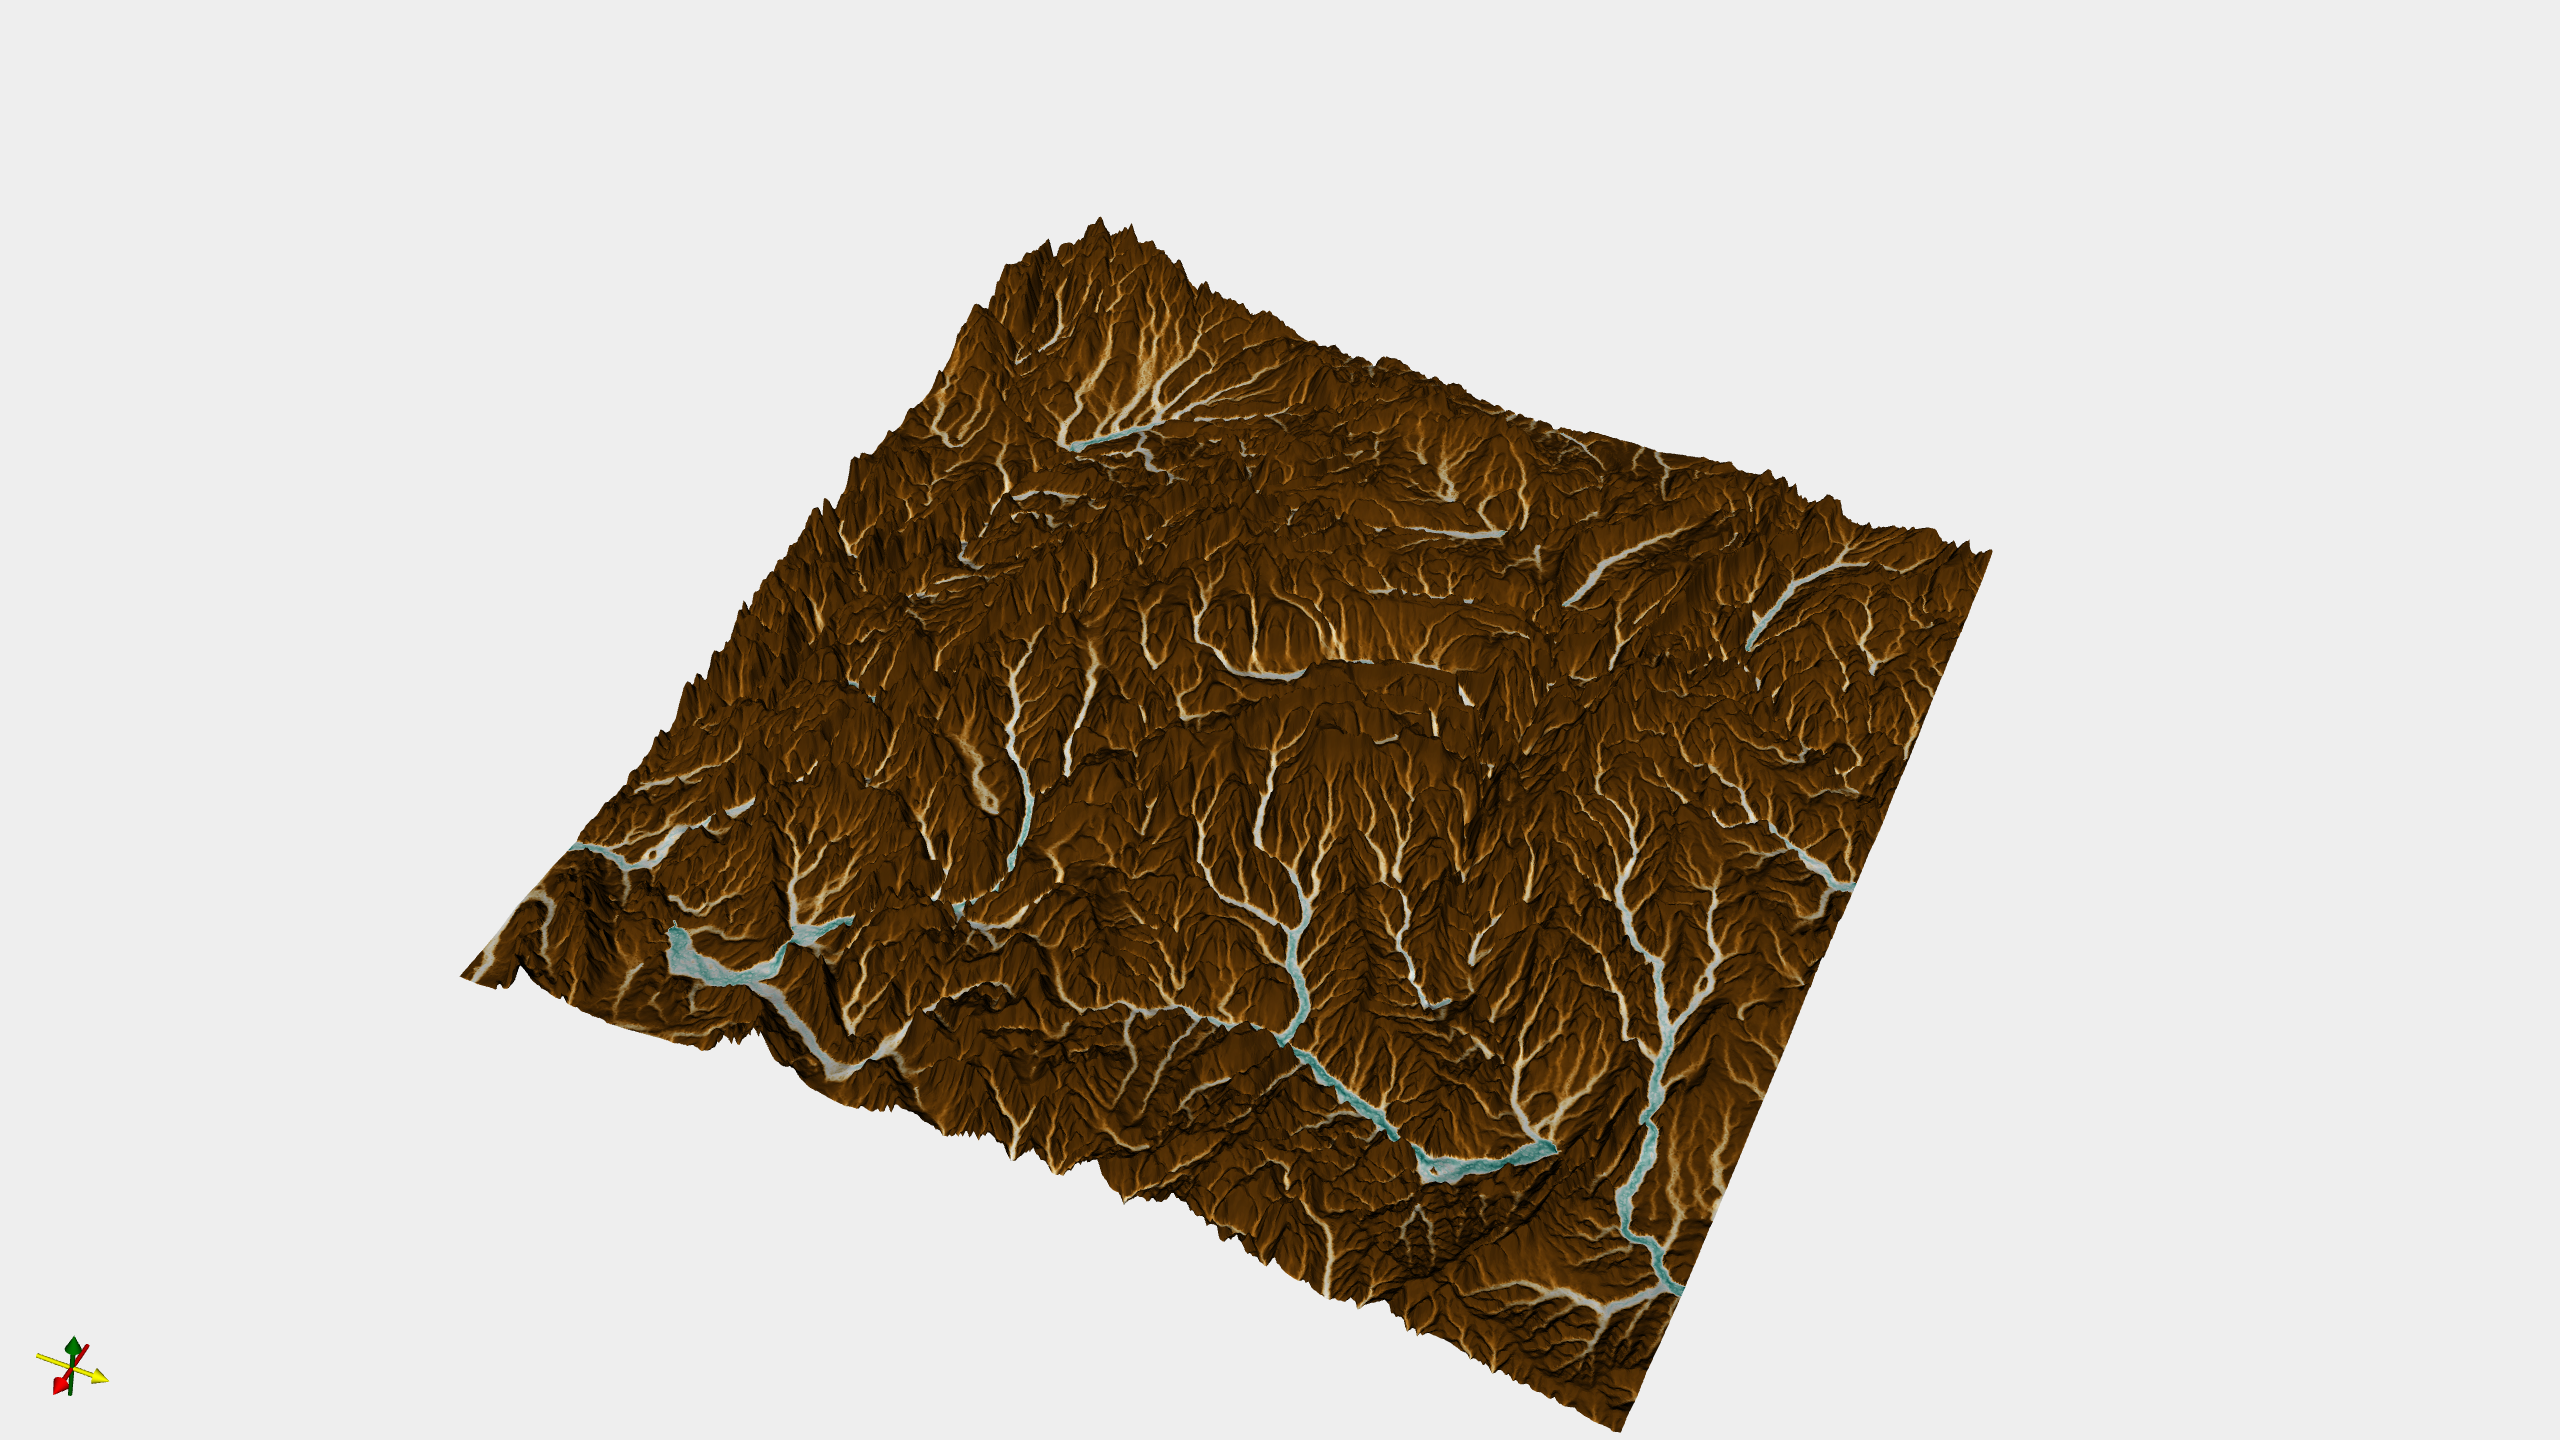
\includegraphics[width=.98\textwidth]{./figures/ch3-bergantes-flow.png}
\end{minipage}
\end{minipage}
\caption{Example model evolution of the Riu Bergantes and surrounding area in the Iberian Massif, Spain. The model fLEM (\url{https://github.com/johnjarmitage/flem}) is run on the SRTM DEM that includes the Riu Bergantes in the bottom corner. The model is run as described in \cite{armitage-2019} for 20\,kyrs, for which the flow field is displayed on the right. No colour bars are shown, as this model is simply a demonstration of the idea rather than a full simulation.}
\label{fg:bergnates}
\end{figure}

To better understand the key processes I am involved in a large project where we plan to compare multiple LEMs on one single catchment, the Riu Bergantes in Spain (Figure \ref{fg:bergantes}). The aim is to take a series of different LEMs: fLEM \citep{armitage-2019}, TISC \citep{garcia-castellanos-2002}, LAPSUS \citep{schoorl-etal-2000}, and CAESAR-Lisflood \citep{coulthard-etal-2013}, and apply them to the same region and explore how they differ in terms of predicted topography and sediment flux.

Sensitivity analysis\dots
  

\section{Long-Term Research Perspectives}

Couple groundwater and landscape evolution.

Develop a reduced complexity model of landscape evolution that can be used to help understand how landscape will react to the coming climate crisis.

\emph{Groundwater and Landscape Evolution, and future climate change.}
